\documentclass[a4paper,12pt]{article}


\usepackage[T1]{fontenc}
\usepackage[utf8]{inputenc}
\usepackage[frenchb]{babel}

\usepackage{graphicx}

\title{Compte rendu de travaux pratiques\\ \small ou un meilleur titre}
\author{Vincent Denechaud, Olivier Maillet, Alice Odier, Félix Tora}
\date{Vendredi 24 janvier 2014}






\begin{document}

\maketitle

Voilà où on pourrait mettre l'introduction, sur les techniques MEB sans trop en faire.


\section{Ici ce serait la première partie}

Pourquoi pas sur l'éponge de Nickel ?

\section{On pourrait mettre une deuxième partie ici}

Sur un autre échantillon.

\vspace{5cm}

Et imaginer d'autres parties, des sous parties et des jolies images comme sur la figure \ref{fig:ni_er_amb}.

\begin{figure}
\centering
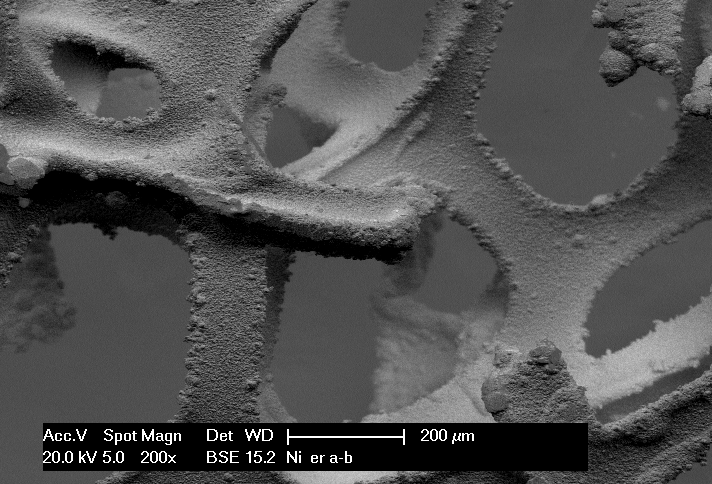
\includegraphics[width = 0.7 \textwidth]{images/ni_er_amb.png}
\caption{Avec une jolie légende en prime}
\label{fig:ni_er_amb}
\end{figure}

\section*{Conclusion}

Et puis tout à la fin on pourrait mettre une petite conclusion aux petits oignons.


\end{document}
